With the high level function of the tachometer components explained, this section describes the hardware and software design process of the tachometer. 

\subsection{Hardware}
Before delving into the software controlling the tachometer or the methods and algorithms, the hardware must first be presented to give context to the software design. This order of presentation is not perfect, as many hardware design decisions were influenced by the presence of the signal processor and its selection of peripherals. A complete schematic is given in Appendix~\ref{app:schem}. The schematic is too large to fit on a single page and remain readable, so it is broken into four separate pages. Figure~\ref{fig:block_schem} serves to illustrate the connection between the different pages of the schematic.

\begin{figure}[H]
    \centering
    \includegraphics[width=.8\textwidth]{schem_block}
    \caption{Diagram of schematic page relationship}
    \label{fig:block_schem}
\end{figure}

The power supply and sensor conditioner are built on separate PCBs from the tachometer, as they are required to meet specifications, but not essential to operation of the tachometer's primary function - measuring RPM. While a power supply must be present in order for the tachometer to function, the designed power supply is not a requirement. The power supply could be replaced with an off-the-shelf switching  or linear regulator, such as the LM7805.

\subsubsection{Power Supply}
\label{sec:ps}
The power supply is a DC-DC converter that reduces the nominal 12V of the battery to a stable 5V for the tachometer. Presented is a justification of the output voltage choice and engineering decisions behind component selection.

\paragraph{Output Voltage}
The initial specified output voltage of the power supply was 3.3V, however during the design process it was determined a higher voltage of 5V would improve performance when driving the gauge. As is discussed in detail in Section~\ref{sec:gauge}, the gauge is controlled by driving current through the coils in a specific manner. In order to drive enough current through the gauge coil, a large enough rail voltage must be present for the gauge driver circuitry. 

Since the gauge of the customer's boat is not removable from the boat and unavailable for testing, measurements were taken to characterize the gauge and a similar gauge was used for testing purposes. The boat gauge had a measured impedance of 230$\Omega$ and the test gauge had a measured impedance of 80$\Omega$. The low impedance test gauge was able to be driven reliably with the lower rail voltage of 3.3V. However, the higher impedance gauge on the boat results in a coil current of only 14mA at maximum differential. A low coil current in the gauge risks unreliable performance. For this reason, the rail voltage was increased to ensure reliable operation.

To comply with contract specifications, the designed power supply was made to be adjustable to either 3.3V or 5V, and the tachometer was designed to operate at both voltage levels. The tachometer is recommended to be run at the higher 5V.

\paragraph{Design}
A DC-DC converter was built to reduce the 12V battery to 5V for the tachometer circuitry. The DC-DC converter was designed with the Texas Instruments LM2675 Simple Switcher. A simple switcher was used for a few reasons: simplicity to construct, documentation and parts availability, and the built-in feedback to ensure stable output voltage. Shown below in Figure~\ref{fig:lm2675_ps} is the generic schematic as suggested by the datasheet. 

\begin{figure}[H]
    \centering
    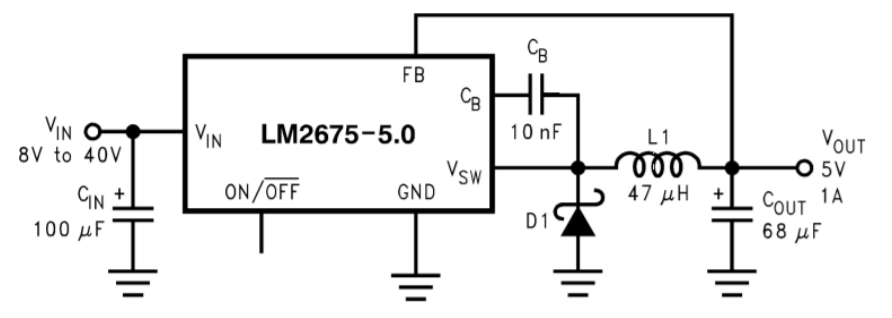
\includegraphics[width=.75\textwidth]{lm2675_schem}
    \caption{Power supply schematic from datasheet~\cite{lm2675}}
    \label{fig:lm2675_ps}
\end{figure}

The suggested schematic is for a 5V output DC-DC converter. During the prototyping process, a 100uH inductor value was selected for availability reasons. Calculations indicate that a minimum inductor value would be 47uH. The minimum inductor value is rarely an ideal choice, as manufacturing variations could result in the DC-DC converter failing to remain in continuous current mode. The inductor stores energy, acting as a current source for the output when the switcher is "off". If the inductor cannot store enough charge, the DC-DC converter may not be able to supply enough current and the output voltage will fluctuate. The inductor selection chart from the LM2675 datasheet is shown below in Figure~\ref{fig:inductor}.

\begin{figure}[H]
    \centering
    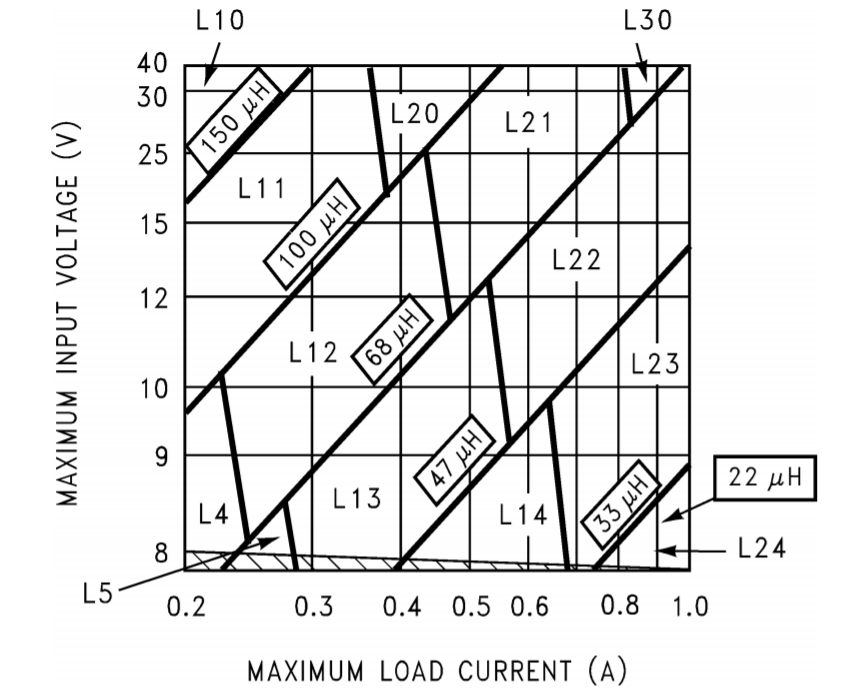
\includegraphics[width=.52\textwidth]{ps_ind}
    \caption{TI simple switcher inductor selection chart~\cite{lm2675}}
    \label{fig:inductor}
\end{figure}

The chart is specifically intended for 5V implementations of the LM2675. Similar charts are present for other voltage levels. Despite datasheet tables and current ripple calculations suggesting the use of a 68uH inductor, the 100uH was used in the final design. A slightly higher inductor value than is recommended typically does not negatively impact power supply performance. The inductor stores energy while the switcher is on, and then dumps that energy when the switcher is off. For this reason, a larger inductor allows more current to be drawn, without risking discontinuous operation. As per datasheet recommendation, a low equivalent series resistance (ESR), 100uF capacitor was added to the input node of the power supply to reduce transients into the converter. The Schottkey diode, D1 in Figure~\ref{fig:lm2675_ps}, needed to be capable of switching quickly in order to keep up with the Simple Switcher's internal frequency of 260kHz. It is also important to use a Schottkey diode due to their low forward voltage drop. This low drop allows the diode to turn on sooner, creating a more stable DC output.

Output capacitors were also needed to smooth out the ripple created by the switching of the LM2675 chip. Similarly to inductor selection, the datasheet had charts to aid in the determination of output capacitor values. The output capacitors were selected to be low ESR ceramic capacitors. When designing the PCB, space for five capacitors was allocated for each decade ranging from 100uF down to 10nF to ensure output ripple could be kept below the specified 100mV. Each decade of capacitor filters a different frequency range, thus implementing more decades allows for better overall filtering.

To make the output adjustable, the LM2675-ADJ was used along with a potentiometer based resistor network on the feedback line. Figure~\ref{fig:feedback} below shows the recommended LM2675-ADJ with feedback network.

\begin{figure}[H]
    \centering
    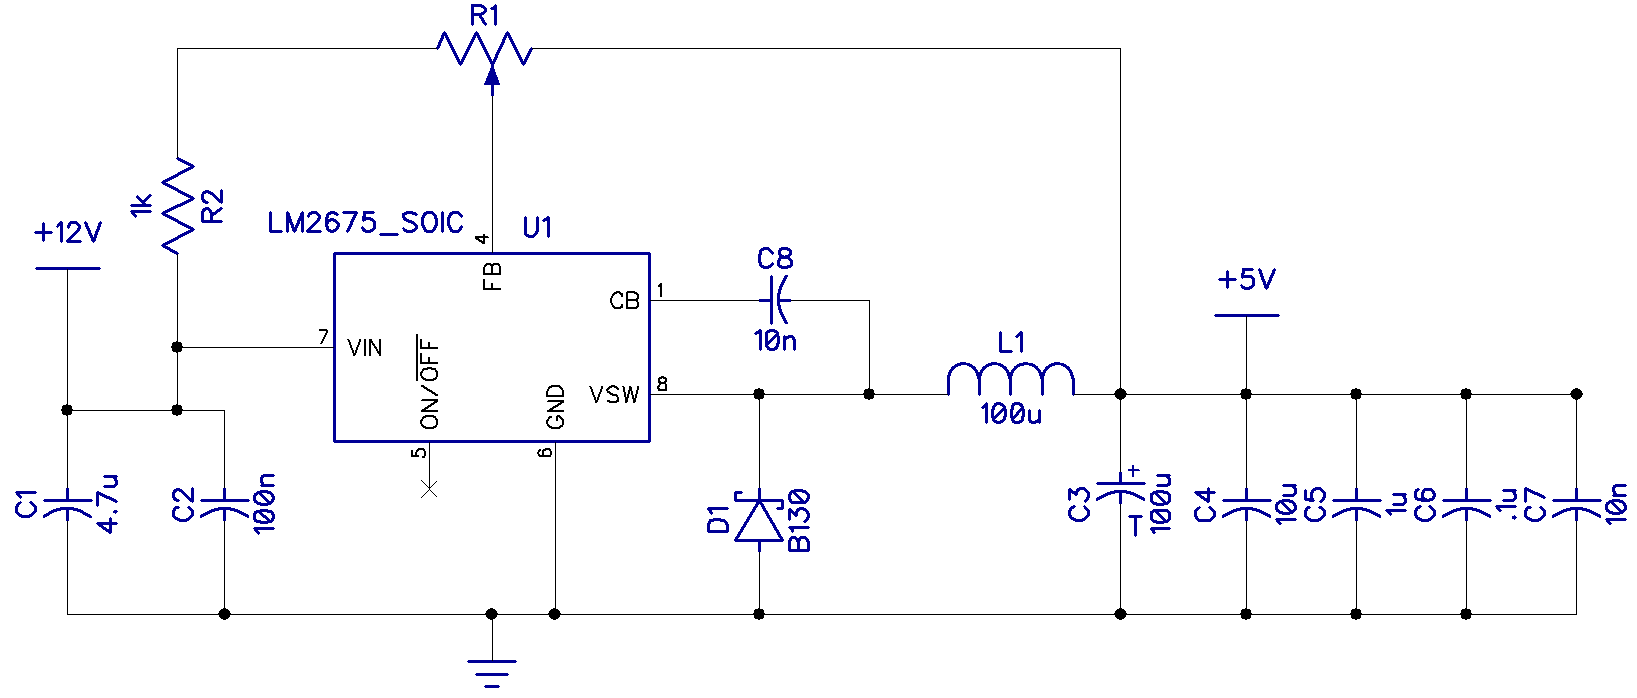
\includegraphics[width=\textwidth]{ps}
    \caption{Adjustible power supply with feedback network}
    \label{fig:feedback}
\end{figure}

The position of the potentiometer, R1, in the schematic determines the output voltage of the regulator. By adjusting the potentiometer, the output voltage can be adjusted as needed.

\subsubsection{Ignition Signal Conditioner}
The ignition signal conditioner was one of the primary challenges presented by this project. The ignition system of the engine employs a coil to gather charge, which is then dissipated to make the spark plug ignite the fuel in the engine cylinder. The process of building and releasing charge produces a noisy ignition signal that needs to be measured by the tachometer to determine engine RPM. The ISC filters out the noise and prevents large magnitude transients from destroying the tachometer circuitry. If the tachometer is not sufficiently protected against noise and large magnitude transients, the system would not work reliably.

\paragraph{Ignition System} %%%%%%%%%%%%%%%%%%%%%%% IGNITION
\label{par:ignition}

The ignition system on a gasoline engine fires the spark plugs to make the engine run. Figure~\ref{fig:ignition} shows the ignition system typically used on older gasoline engines, such as that used in the 1988 Celebrity Champion.



\begin{figure}[H]
    \centering
    \includegraphics[width=\textwidth]{ignition}
    \caption{Engine ignition system}
    \label{fig:ignition}
\end{figure}

When the ignition switch is turned on, the positive side of the ignition coil is connected to 12V. A distributor is the device on an engine that contains the points and fires the spark plugs at the correct time. As the distributor turns, the points close. Closing of the points connects the negative side of the ignition coil to ground causing current to flow though the coil. When current flows through the coil, a magnetic field is built up inside the windings. As the distributor keeps turning, the points open again, releasing the magnetic field in the form of high voltage to the spark plugs. The condenser, or capacitor, keeps voltage from arcing across the contacts of the points. Figure~\ref{fig:boat_noise} illustrates one of the biggest challenges of hardware design in this project: voltage spikes.

\begin{figure}[H]
    \centering
    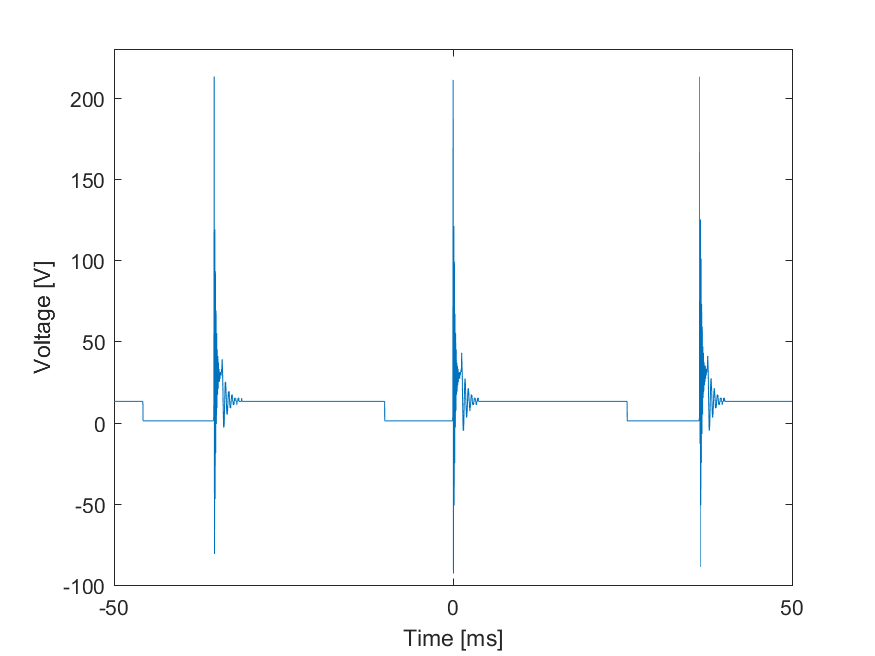
\includegraphics[width=.8\textwidth]{boat_raw}
    \caption{Ignition signal from Celebrity Champion}
    \label{fig:boat_noise}
\end{figure}

 The signal processing unit can only tolerate a 5V signal, however, when high voltages are created using a coil of wire, large voltage spikes and high amounts of noise are created. As shown in Figure~\ref{fig:boat_noise}, these voltage spikes can be in excess of 200V.

\paragraph{Design}
The signal shown in Figure~\ref{fig:boat_noise}, needs to have the voltage spikes removed. It is crucial that this be done in a robust manner to ensure long-term reliability of the tachometer. The bulk of this task can be handled by a few passive components. First, a resistive voltage divider reduces the logic level from 12V to 5V. A pair of diodes clamps the signal, preventing it from exceeding the positive rail voltage or dipping below the reference rail voltage. The resistive voltage divider also acts as a current limit, protecting the diodes from damage. Finally, a capacitor creates a low pass filter. This partial circuit is shown below in Figure~\ref{fig:clamp_filter}.

\begin{figure}[H]
    \centering
    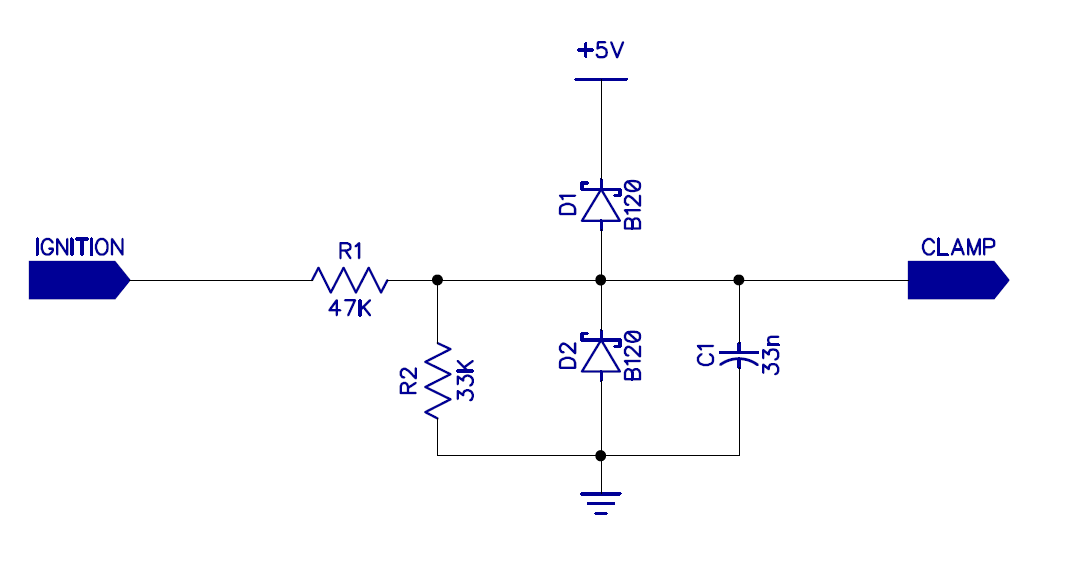
\includegraphics[width=.85\textwidth]{clamp}
    \caption{Partial input filter circuit}
    \label{fig:clamp_filter}
\end{figure}

The resistor values were chosen such that they created a voltage divider with a ratio of approximately $5/12$ and had a total resistance over 50k$\Omega$. The voltage divider current limits the signal while stepping down the logic level. To effectively clamp the signal to the supply voltage, fast switching, low voltage drop diodes were needed. Low voltage drop was needed to allow the signal to be clamped to a voltage close to that of the supply. Fast switching was needed to change state at a speed which matches that of the high frequency noise. Schottkey diodes have all of these characteristics. The capacitor selection process involved calculating the maximum frequency the ignition signal could reasonably reach and then placing the cutoff frequency of the low pass filter slightly above that.

The maximum frequency of the ignition signal is 300Hz (corresponding to 9000 engine RPM). With a maximum input frequency of 300Hz, a cutoff frequency above 1kHz does not cause interference with the ignition signal integrity. The low pass filter created by R1, R2, and C1 places a cutoff frequency around 1.56kHz.

Figure~\ref{fig:diode} shows the ignition signal after passing through the partial conditioning circuit.
\begin{figure}[H]
    \centering
    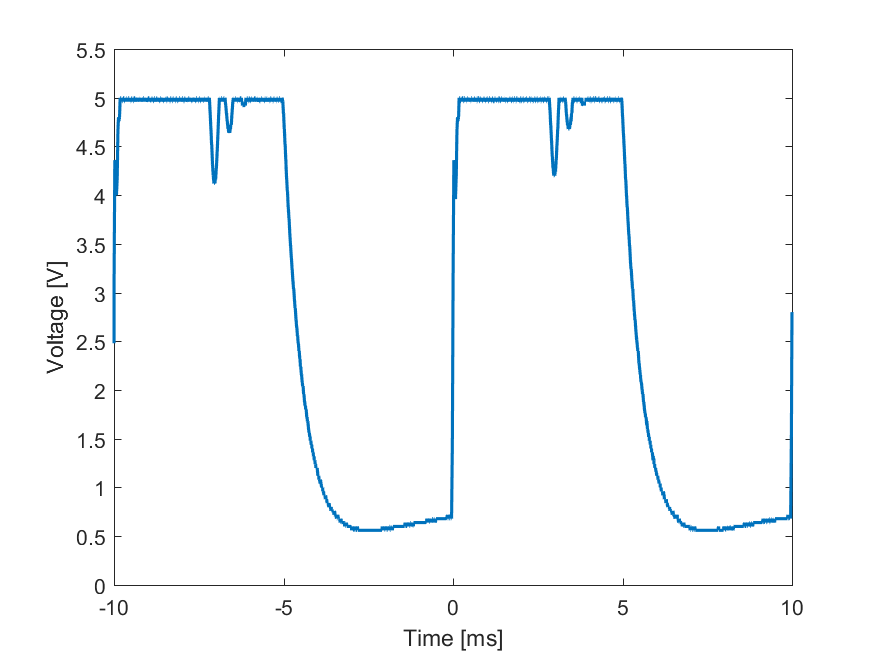
\includegraphics[width=.75\textwidth]{diode}
    \caption{Ignition signal after clamping and filtering}
    \label{fig:diode}
\end{figure}

Most noise is removed, and the output resembles a square wave. To further condition the signal, it was fed into a comparator to generate a clean square wave for the signal processor. To increase reliability, the comparator was configured to use hysteresis. Since configuring hysteresis lowers the input impedance of the comparator, the output of the clamp was passed through an operational amplifier unity gain buffer before being passed to the comparator. The additional ignition conditioning circuitry is shown in Figure~\ref{fig:comp} below.

\begin{figure}[H]
    \centering
    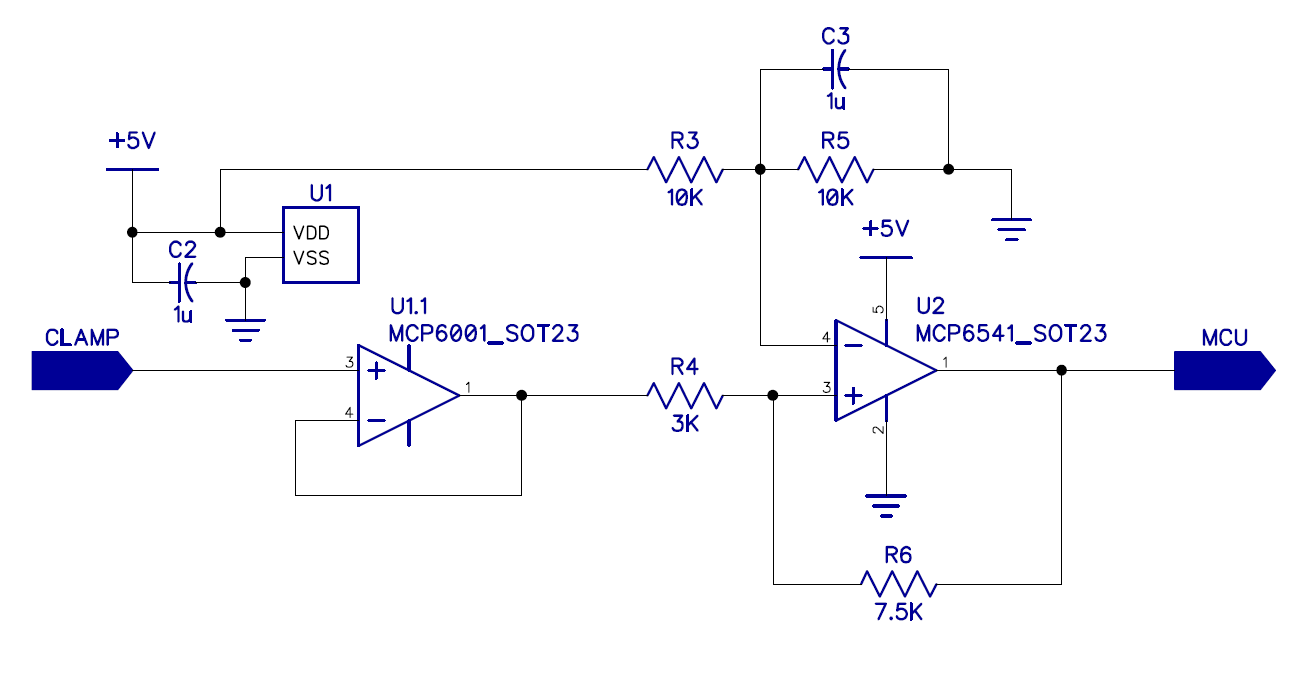
\includegraphics[width=.9\textwidth]{comp}
    \caption{Ignition signal current buffer and comparator}
    \label{fig:comp}
\end{figure}

To determine the resistor values to set the hysteresis of the comparator,  Equations~\ref{eq:hist1}~and~\ref{eq:hist2} were adapted from the datasheet\cite{mcp6541} for this application.

\begin{equation}
\label{eq:hist1}
    V_{TLH} = 2.5V(1+\frac{R_4}{R_6}) - V_{OL}(\frac{R_4}{R_6})
\end{equation}
\begin{equation}
\label{eq:hist2}
    V_{THL} = 2.5V(1+\frac{R_4}{R_6}) - V_{OH}(\frac{R_4}{R_6})
\end{equation}

In the equations above, $V_{OH}$ and $V_{OL}$ are the desired high and low output voltages, respectively. $V_{THL}$ and $V_{TLH}$ are the input voltages at which the output will change from high to low, or low to high, respectively. Using the equations above, the resistor values were determined such that an input voltage of 3.5V or more will cause the comparator to switch output from low to high, and an input voltage of 1.5V or less will cause the comparator to switch from high to low. The output of the comparator is shown below in Figure~\ref{fig:conditioned}.

\begin{figure}[H]
    \centering
    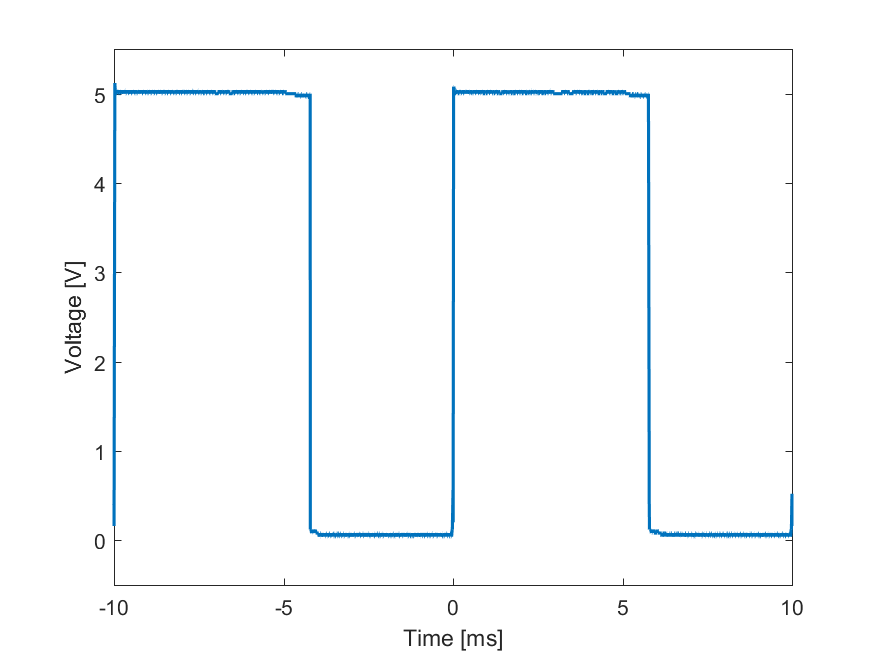
\includegraphics[width=.7\textwidth]{conditioned}
    \caption{Conditioned ignition signal}
    \label{fig:conditioned}
\end{figure}

With the ignition signal conditioned to a square wave, the signal processor can now accurately measure the frequency with a digital pin. The filtering and and buffering done by the ignition signal conditioner also protects the rest of the circuit from the noise introduced by the ignition signal.

\subsubsection{Gauge Driver} %%%%%%%%%%%%%%%%%%%%%%%%%%%%%%%%%%%%%%%%%%% Gauge Driver %%%%%%%%%%%%%%%%%%%%%%%%%%%%%%%%%%%
\label{sec:gauge} % label to gauge driver for reference elsewhere 
The analog tachometer gauge on the Celebrity Champion is an air core gauge. This section provides discussion on how an air core gauge works, and how a hardware driver was built.
\paragraph{Air Core Gauge}
The air core gauge has three input wires, one at a reference voltage, and two at voltages above and below the reference.

Figure~\ref{fig:aircore} shows a representation of an air core gauge from the LM1819 datasheet.


\begin{figure}[H]
    \centering
    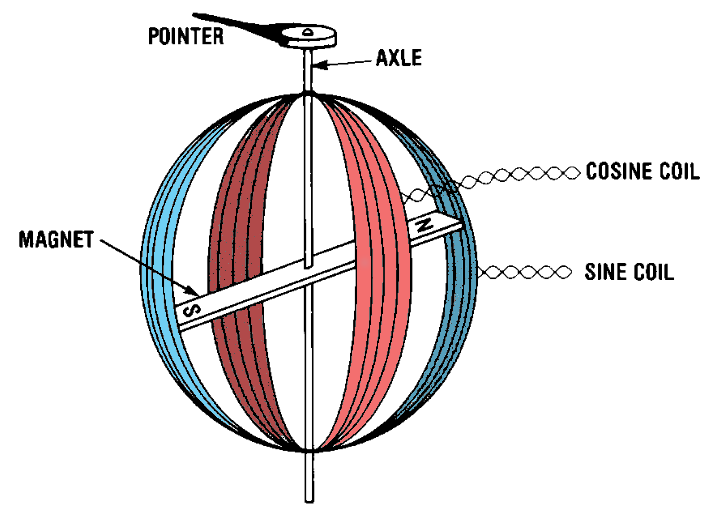
\includegraphics[width=.75\textwidth]{aircore}
    \caption{Diagram of air core gauge~ \cite{lm1819}}
    \label{fig:aircore}
\end{figure}

The air core gauge consists of a magnet and two coils of wire. The pointer is connected to a magnet that lies between the two coils of wire that are 180$^{\circ}$ degrees apart. When a voltage is applied to the coils, a magnetic field is created that moves the magnet, and in turn the pointer. Figure~\ref{fig:tach} shows the relationship between input voltage and pointer deflection.

\begin{figure}[H]
    \centering
    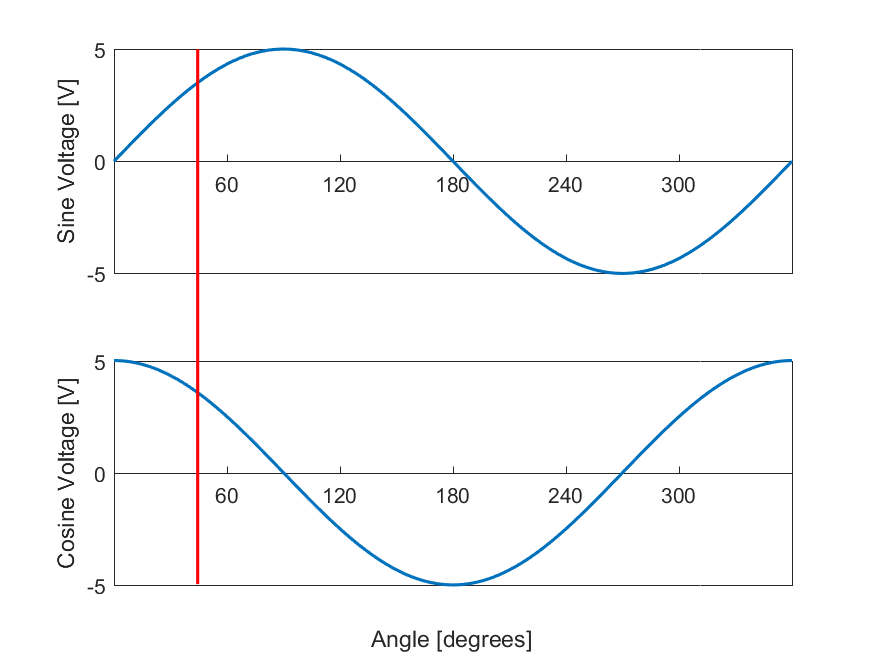
\includegraphics[width=.8\textwidth]{sincos}
    \caption{Input waveform to gauge}
    \label{fig:tach}
\end{figure}

The zero degree line is where both differential inputs to the gauge are at the same voltage and thus the pointer is at zero degrees of deflection. As long as the sine and cosine coils follow the voltage relationship shown in Figure~\ref{fig:tach}, the pointer turns smoothly in a circle.
\paragraph{Design}
Due to the impedance of the coils in the gauge on the Celebrity Champion, the reference voltage was chosen to be 5V and the rail voltage was 10V. This was done so that the peak current flowing through the coils was around 22mA. If the 3.3V logic level was used, a peak current of only about 14mA would flow through the coils. Testing showed that a peak current of less than 10mA was not sufficient for reliable gauge operation, and the 14mA of the 3.3V logic level was too close to this lower limit. Since reliability is a large concern for this project, a higher logic level was used.

Since the output from the signal processor is only 5V, a buffering level shifter was built. The cosine coil driver is shown in Figure~\ref{fig:buflevel}, an identical one was also built for the sine coil. 

\begin{figure}[H]
    \centering
    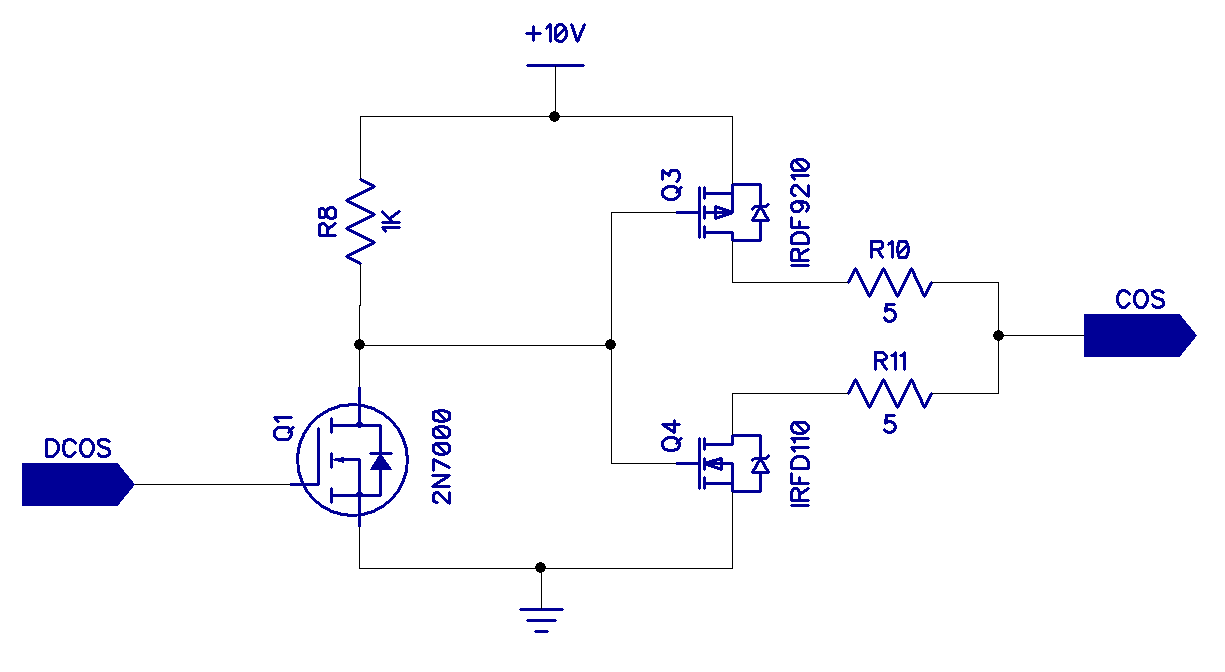
\includegraphics[width=\textwidth]{gauge_driver}
    \caption{Buffering level shifter to drive tachometer}
    \label{fig:buflevel}
\end{figure}


A 0V input to DCOS on the level shifter creates an output of 0V, and an input of 5V creates an output of 10V. The result is a 5V center voltage to the tachometer with a 0V to 10V on the differential inputs of the air core gauge.

%%%%%%%%%%%%%%%%%% SOFTWARE STUFF HERE
\subsection{Software}
This section discusses the software running on the signal processor.
The main loop checks for new raw input values and converts them human readable information. New input values include: ADC values from engine sensors, RPM values from the ignition signal, and request for programming mode. After processing the inputs, the main loop outputs the values to either the Gauge Driver, or the detachable display. Figure~\ref{fig:softbd} shows the software block diagram.
\begin{figure}[H]
    \centering
    \includegraphics[width=.75\textwidth]{softBD}
    \caption{Software block diagram of Signal Processor}
    \label{fig:softbd}
\end{figure}

The software block diagram helps understand how the signal processor works. The interrupts set flags that the main loop checks for each time around. If a flag is set, the main loop performs a certain task. For example, when the ignition input interrupt is triggered, an algorithm is run to determine the frequency of the input signal. The input frequency is then converted into an RPM value to be sent to the gauge driver or the digital display.

\subsubsection{Programming Mode} %%%%%%%%%%%%%%%%%% PROGRAMMING MODE
Programming mode is for calibrating the tachometer for a particular installation. A couple parameters need to be set: the range of the analog gauge, and the analog input values for the engine sensors. A serial interrupt alerts the main loop if a user has requested programming mode. After calibration has been performed, the calibration values are stored to a data structure in the electronically erasable programmable read only memory.

\subsubsection{ADC} %%%%%%%%%%%%%%%%%% ADC
The engine sensors connect to the ADC inputs on the microcontroller. The ADC produces values between 0 and 1023, the ADC routine then converts these into human readable information. First, the main loop requests an ADC reading for a certain sensor input. Once a request is made, the ADC interrupt is turned on. After the ADC value is recorded, the ADC interrupt triggers the ADC calculation, which then converts the input to a human readable information using the values stored in the configuration structure.


\subsubsection{Conditioned Ignition Input} %%%%%%%%%%%%%%%%%% TACH INPUT
To calculate the engine RPM, the conditioned ignition input is connected to a hardware interrupt pin on the microcontroller. Every time a rising edge is detected on the input, the conditioned ignition interrupt is triggered. When the interrupt is triggered, it reads the value of Timer~1. The microcontroller runs at 8MHz, and timer~1 is configured with a divide by 8 prescaler, meaning timer~1 is counting  microseconds. The input interrupt saves the value of timer~1 to a global variable and resets the timer.

The RPM calculation block then looks at the value of the timer and uses that value to calculate the input frequency of the ignition input, which can then be correlated to the engine RPM. Since timer~1 is a 16-bit timer, the slowest input period that can be calculated in 65535 microseconds, or about 15Hz. If the input frequency is lower than 15Hz, Timer~1 overflow interrupt is triggered and alerts the RPM calculation block allowing frequencies with a period as high as 65535 + 65535 = 131072 microseconds, or 7.6Hz to be calculated. With a speed that low, the engine is assumed to be stopped, and the output RPM signal is set to zero.

After determining the input frequency, the RPM calculation block needs to convert frequency to RPM. Equation~\ref{eqn:RPM} shows the calculation for a four cylinder, for stroke engine.
\begin{equation}
    \label{eqn:RPM}
    RPM = 30*Hz
\end{equation}
After the RPM is calculated, the value is saved to be processed by the gauge driver.

\subsubsection{Gauge Output} %%%%%%%%%%%%%%%%%% TACH OUTPUT
The gauge output driver must interface with the hardware output driver described in Section~\ref{sec:gauge}. Since the microcontroller used in this project does not have a digital to analog converter, it uses pulse width modulation (PWM) to simulate an analog voltage with a pulsed square wave. A 31kHz PWM frequency was used in this project because it is higher than human hearing, thus avoiding a high pitch humming from the air core gauge.

Section~\ref{sec:gauge} discussed driving the gauge with two sine waves, however the gauge driver software only changes the value of one input at a time. Figure~\ref{fig:scPWM} shows the curve used in software.

\begin{figure}[H]
    \centering
    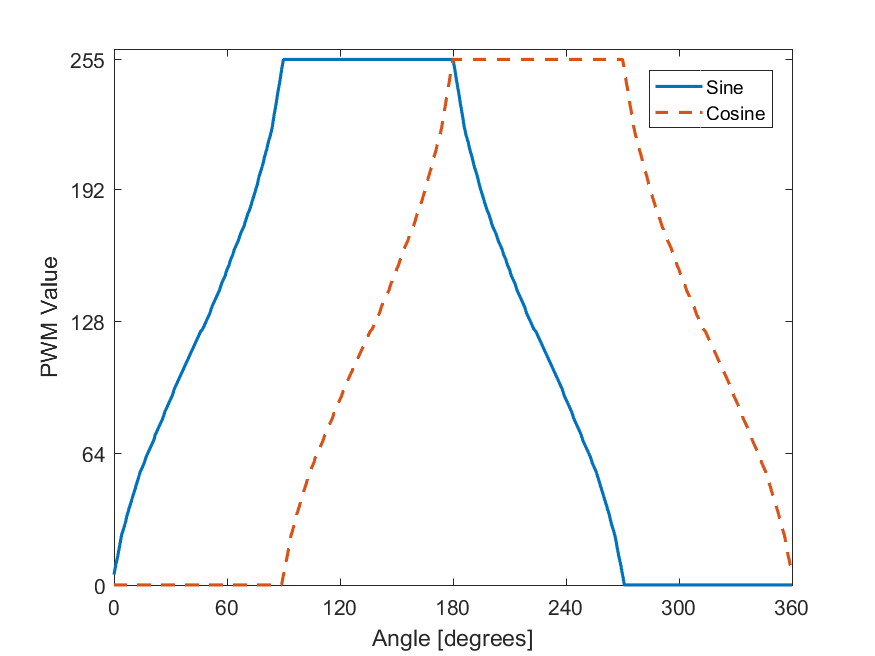
\includegraphics[width=\textwidth]{sinarr}
    \caption{Sine and cosine curve used for gauge driver}
    \label{fig:scPWM}
\end{figure}

As discussed before, the pointer on the gauge still moves linearly, however the driver uses a lookup table with a tangent curve. The result is that one output, either sine or cosine, is always either high or low, and the other input changes with pointer deflection angle. This method of gauge control was easier and faster to design in software than changing both inputs at the same time.

\subsubsection{Display Driver} %%%%%%%%%%%%%%%%%% DISPLAY
The detachable display used in this project is a Hitachi HD44780 16 character by 2 line display. The display is used for showing values of engine sensors read in by the ADC, and the RPM of the engine. The display is hot swappable, meaning it can be connected or disconnected from the tachometer at any time. Hot swapping is a useful feature for debugging errors and checking on the health of an engine.

A device driver was written in order to use the display. Due to limited number of available outputs on the microcontroller, the display was used in 4-bit mode, meaning sending a character, an 8-bit value, takes two write cycles. First, the display is initialized which tells the display where the first character of each line starts and what font to use. After initialization a print function writes data out to the display; however, due to timing requirements, large delays between sending each piece of information exist. Rather than sit in an empty loop, the driver makes use of timers. When the display driver requires a delay, timer~2 is activated and the display driver lets other tasks run. When Timer~2 interrupts, the display driver sends the next piece of information and goes back to waiting. Using an interrupt based driver is much more efficient than dead loops because it allows other tasks, such as calculating RPM and reading ADC values, to continue.

The initialization function must also be called when the display is hot swapped. To achieve this, an extra pin was added to the connector between the display and the tachometer. The extra pin is connected to a hardware interrupt that, when triggered, initializes the display.